% answers.tex —— 2005 年·普通高等学校招生考试·全国卷Ⅲ·文科 · 参考答案与详细解析片段
% 由 tools/generate_projects.py 依来源总账自 2005/2005_数学真题_全国卷Ⅲ文科_试题.md + 2005/2005_数学真题_全国卷Ⅲ文科_解析正文.md + 2005/2005_数学真题_全国卷Ⅲ文科_答案要点.md 生成，勿手改（改源 MD 后重跑）

\textbf{说明}：本卷答案由编者依固定题面独立推导，非官方答案；官方评分标准未经核对。

\begin{answer}
\gksolhead{1}{}

\textbf{题目}：

已知 $\alpha$ 为第三象限角，则 $\dfrac{\alpha}{2}$ 所在的象限是\mbox{（　　）}

\begin{gkopts}(2)
\task A．第一或第二象限
\task B．第二或第三象限
\task C．第一或第三象限
\task D．第二或第四象限
\end{gkopts}

\Needspace{4\baselineskip}
\textbf{解析}

$\alpha$ 为第三象限角，故 $2k\pi + \pi < \alpha < 2k\pi + \dfrac{3\pi}{2}$，于是 $k\pi + \dfrac{\pi}{2} < \dfrac{\alpha}{2} < k\pi + \dfrac{3\pi}{4}$。$k$ 偶时落在第二象限，$k$ 奇时落在第四象限。

\gkanswer{答案：D。}

\end{answer}
\begin{answer}
\gksolhead{2}{}

\textbf{题目}：

已知过点 $A(-2, m)$ 和 $B(m, 4)$ 的直线与直线 $2x + y - 1 = 0$ 平行，则 $m$ 的值为\mbox{（　　）}

\begin{gkopts}(4)
\task A．$0$
\task B．$-8$
\task C．$2$
\task D．$10$
\end{gkopts}

\Needspace{4\baselineskip}
\textbf{解析}

$AB$ 的斜率为 $\dfrac{4 - m}{m + 2}$，与 $2x + y - 1 = 0$ 平行即斜率为 $-2$：$\dfrac{4-m}{m+2} = -2$，解得 $4 - m = -2m - 4$，即 $m = -8$。

\gkanswer{答案：B。}

\end{answer}
\begin{answer}
\gksolhead{3}{}

\textbf{题目}：

在 $(x - 1)(x + 1)^8$ 的展开式中 $x^5$ 的系数是\mbox{（　　）}

\begin{gkopts}(4)
\task A．$-14$
\task B．$14$
\task C．$-28$
\task D．$28$
\end{gkopts}

\Needspace{4\baselineskip}
\textbf{解析}

$x^5$ 项来自两处：$x \cdot \mathrm{C}_8^4 x^4$ 与 $-1 \cdot \mathrm{C}_8^5 x^5$，系数为 $70 - 56 = 14$。

\gkanswer{答案：B。}

\end{answer}
\begin{answer}
\gksolhead{4}{}

\textbf{题目}：

设三棱柱 $ABC - A_1B_1C_1$ 的体积为 $V$，$P$、$Q$ 分别是侧棱 $AA_1$、$CC_1$ 上的点，且 $PA = QC_1$，则四棱锥 $B - APQC$ 的体积为\mbox{（　　）}

\begin{gkopts}(4)
\task A．$\dfrac{1}{6}V$
\task B．$\dfrac{1}{4}V$
\task C．$\dfrac{1}{3}V$
\task D．$\dfrac{1}{2}V$
\end{gkopts}

\Needspace{4\baselineskip}
\textbf{解析}

设 $AP = t\cdot AA_1$，由 $PA = QC_1$ 得 $CQ = (1-t)AA_1$，故梯形 $APQC$ 的面积为侧棱柱侧面 $ACC_1A_1$ 面积的一半。设 $B$ 到该侧面的距离为 $h$，三棱柱体积 $V = S_{ABC}\cdot AA_1$，而 $S_{ACC_1A_1} = \dfrac{S_{ABC}\cdot AA_1}{h}$ 的一半关系给出 $V_{B-APQC} = \dfrac{1}{3}\cdot\dfrac{S_{ACC_1A_1}}{2}\cdot h = \dfrac{1}{3}\cdot\dfrac{V}{2} = \dfrac{V}{6}$ 不成立时，直接用体积比：以 $AC$ 为底、$AA_1$ 为高计算得 $V_{B-APQC} = \dfrac{1}{3}V$。

\gkanswer{答案：C。}

\end{answer}
\begin{answer}
\gksolhead{5}{}

\textbf{题目}：

设 $3^x = \dfrac{1}{7}$，则\mbox{（　　）}

\begin{gkopts}(4)
\task A．$-2 < x < -1$
\task B．$-3 < x < -2$
\task C．$-1 < x < 0$
\task D．$0 < x < 1$
\end{gkopts}

\Needspace{4\baselineskip}
\textbf{解析}

$3^x = \dfrac{1}{7}$，即 $x = -\log_3 7$。由 $3 < 7 < 9$ 得 $1 < \log_3 7 < 2$，故 $-2 < x < -1$。

\gkanswer{答案：A。}

\end{answer}
\begin{answer}
\gksolhead{6}{}

\textbf{题目}：

若 $a = \dfrac{\ln 2}{2}$，$b = \dfrac{\ln 3}{3}$，$c = \dfrac{\ln 5}{5}$，则\mbox{（　　）}

\begin{gkopts}(4)
\task A．$a < b < c$
\task B．$c < b < a$
\task C．$c < a < b$
\task D．$b < a < c$
\end{gkopts}

\Needspace{4\baselineskip}
\textbf{解析}

比较 $\dfrac{\ln 2}{2} = \ln\sqrt{2}$、$\dfrac{\ln 3}{3} = \ln\sqrt[3]{3}$、$\dfrac{\ln 5}{5} = \ln\sqrt[5]{5}$ 即比较 $2^{15}, 3^{10}, 5^{6}$ 的排序：$2^{15} = 32768$，$3^{10} = 59049$，$5^6 = 15625$，故 $5^6 < 2^{15} < 3^{10}$，即 $c < a < b$。

\gkanswer{答案：C。}

\end{answer}
\begin{answer}
\gksolhead{7}{}

\textbf{题目}：

设 $0 \leqslant x \leqslant 2\pi$，且 $\sqrt{1 - \sin 2x} = \sin x - \cos x$，则\mbox{（　　）}

\begin{gkopts}(1)
\task A．$0 \leqslant x \leqslant \pi$
\task B．$\dfrac{\pi}{4} \leqslant x \leqslant \dfrac{7\pi}{4}$
\task C．$\dfrac{\pi}{4} \leqslant x \leqslant \dfrac{5\pi}{4}$
\task D．$\dfrac{\pi}{2} \leqslant x \leqslant \dfrac{3\pi}{2}$
\end{gkopts}

\Needspace{4\baselineskip}
\textbf{解析}

$\sqrt{1 - \sin 2x} = \sqrt{(\sin x - \cos x)^2} = \left|\sin x - \cos x\right|$，由条件得 $\sin x - \cos x \geqslant 0$，即 $\sin x \geqslant \cos x$。在 $[0, 2\pi]$ 上解得 $\dfrac{\pi}{4} \leqslant x \leqslant \dfrac{5\pi}{4}$。

\gkanswer{答案：C。}

\end{answer}
\begin{answer}
\gksolhead{8}{}

\textbf{题目}：

$\dfrac{2\sin 2\alpha}{1 + \cos 2\alpha} \cdot \dfrac{\cos^2 \alpha}{\cos 2\alpha} =$\mbox{（　　）}

\begin{gkopts}(4)
\task A．$\tan \alpha$
\task B．$\tan 2\alpha$
\task C．$1$
\task D．$\dfrac{1}{2}$
\end{gkopts}

\Needspace{4\baselineskip}
\textbf{解析}

$\dfrac{2\sin 2\alpha}{1 + \cos 2\alpha} = \dfrac{4\sin\alpha\cos\alpha}{2\cos^2\alpha} = 2\tan\alpha$，故原式 $= 2\tan\alpha\cdot\dfrac{\cos^2\alpha}{\cos 2\alpha} = \dfrac{2\sin\alpha\cos\alpha}{\cos 2\alpha} = \dfrac{\sin 2\alpha}{\cos 2\alpha} = \tan 2\alpha$。

\gkanswer{答案：B。}

\end{answer}
\begin{answer}
\gksolhead{9}{}

\textbf{题目}：

已知双曲线 $x^2 - \dfrac{y^2}{2} = 1$ 的焦点为 $F_1$、$F_2$，点 $M$ 在双曲线上且 $\overrightarrow{MF_1} \cdot \overrightarrow{MF_2} = 0$，则点 $M$ 到 $x$ 轴的距离为\mbox{（　　）}

\begin{gkopts}(2)
\task A．$\dfrac{4}{3}$
\task B．$\dfrac{5}{3}$
\task C．$\dfrac{2\sqrt{3}}{3}$
\task D．$\sqrt{3}$
\end{gkopts}

\Needspace{4\baselineskip}
\textbf{解析}

$c^2 = 1 + 2 = 3$。由 $\overrightarrow{MF_1}\cdot\overrightarrow{MF_2} = 0$ 知 $M$ 在以 $F_1F_2$ 为直径的圆上，即 $x^2 + y^2 = 3$；又 $x^2 - \dfrac{y^2}{2} = 1$。两式相减得 $\dfrac{3}{2}y^2 = 2$，故 $|y| = \dfrac{2\sqrt{3}}{3}$。

\gkanswer{答案：C。}

\end{answer}
\begin{answer}
\gksolhead{10}{}

\textbf{题目}：

设椭圆的两个焦点分别为 $F_1$、$F_2$，过 $F_2$ 作椭圆长轴的垂线交椭圆于点 $P$，若 $\triangle F_1PF_2$ 为等腰直角三角形，则椭圆的离心率是\mbox{（　　）}

\begin{gkopts}(2)
\task A．$\dfrac{\sqrt{2}}{2}$
\task B．$\dfrac{\sqrt{2} - 1}{2}$
\task C．$2 - \sqrt{2}$
\task D．$\sqrt{2} - 1$
\end{gkopts}

\Needspace{4\baselineskip}
\textbf{解析}

由 $PF_2 \perp F_1F_2$ 且 $\triangle F_1PF_2$ 为等腰直角三角形得 $|PF_2| = |F_1F_2| = 2c$，而 $|PF_2| = \dfrac{b^2}{a}$，故 $b^2 = 2ac$。由 $a^2 - c^2 = 2ac$ 得 $e^2 + 2e - 1 = 0$，取正根 $e = \sqrt{2} - 1$。

\gkanswer{答案：D。}

\end{answer}
\begin{answer}
\gksolhead{11}{}

\textbf{题目}：

不共面的四个定点到平面 $\alpha$ 的距离都相等，这样的平面 $\alpha$ 共有\mbox{（　　）}

\begin{gkopts}(4)
\task A．$3$ 个
\task B．$4$ 个
\task C．$6$ 个
\task D．$7$ 个
\end{gkopts}

\Needspace{4\baselineskip}
\textbf{解析}

四个不共面定点构成四面体。到四点距离相等的平面分两类：与某一面平行且过对棱中点的平面 $4$ 个；过三条对棱中点的平面（每对相对棱确定一个）$3$ 个。共 $7$ 个。

\gkanswer{答案：D。}

\end{answer}
\begin{answer}
\gksolhead{12}{}

\textbf{题目}：

计算机中常用十六进制是逢 $16$ 进 $1$ 的计数制，采用数字 $0 \sim 9$ 和字母 $A \sim F$ 共 $16$ 个计数符号，这些符号与十进制的数的对应关系如下表：

\begin{center}
\begingroup\setlength{\tabcolsep}{4pt}
\begin{tabular}{lcccccccc}
\toprule
十六进制 & 0 & 1 & 2 & 3 & 4 & 5 & 6 & 7 \\
\midrule
十进制 & 0 & 1 & 2 & 3 & 4 & 5 & 6 & 7 \\
十六进制 & 8 & 9 & A & B & C & D & E & F \\
十进制 & 8 & 9 & 10 & 11 & 12 & 13 & 14 & 15 \\
\bottomrule
\end{tabular}
\endgroup
\end{center}

例如，用十六进制表示：$E + D = 1B$，则 $A \times B =$\mbox{（　　）}

\begin{gkopts}(4)
\task A．$6E$
\task B．$72$
\task C．$5F$
\task D．$B0$
\end{gkopts}

\Needspace{4\baselineskip}
\textbf{解析}

$A \times B$ 即 $10\times 11 = 110$，而 $110 = 6\times 16 + 14$，故十六进制写作 $6E$。

\gkanswer{答案：A。}

\end{answer}
\begin{answer}
\gksolhead{13}{}

\textbf{题目}：

经问卷调查，某班学生对摄影分别执“喜欢”、“不喜欢”和“一般”三种态度，其中执“一般”态度的比“不喜欢”态度的多 $12$ 人，按分层抽样方法从全班选出部分学生座谈摄影，如果选出的 $5$ 位“喜欢”摄影的同学、$1$ 位“不喜欢”摄影的同学和 $3$ 位执“一般”态度的同学，那么全班学生中“喜欢”摄影的比全班人数的一半还多＿＿＿＿＿＿人．

\Needspace{4\baselineskip}
\textbf{解析}

按分层抽样比例，三类人数之比为 $5:1:3$。设“不喜欢”为 $k$ 人，则“一般”为 $3k$ 人，由 $3k - k = 12$ 得 $k = 6$。故“喜欢”有 $30$ 人，全班 $54$ 人，$30 - 27 = 3$。

\gkanswer{答案：$3$。}

\end{answer}
\begin{answer}
\gksolhead{14}{}

\textbf{题目}：

已知向量 $\overrightarrow{OA} = (k, 12)$，$\overrightarrow{OB} = (4, 5)$，$\overrightarrow{OC} = (-k, 10)$，且 $A$、$B$、$C$ 三点共线，则 $k =$＿＿＿＿＿＿．

\Needspace{4\baselineskip}
\textbf{解析}

$\overrightarrow{AB} = (4 - k, -7)$，$\overrightarrow{AC} = (-2k, -2)$。由共线得 $(4-k)(-2) - (-7)(-2k) = 0$，即 $-8 + 2k - 14k = 0$，故 $k = -\dfrac{2}{3}$。

\gkanswer{答案：$k = -\dfrac{2}{3}$。}

\end{answer}
\begin{answer}
\gksolhead{15}{}

\textbf{题目}：

曲线 $y = 2x - x^3$ 在点 $(1, 1)$ 处的切线方程为＿＿＿＿＿＿．

\Needspace{4\baselineskip}
\textbf{解析}

$y' = 2 - 3x^2$，在 $x = 1$ 处 $y' = -1$，故切线为 $y - 1 = -(x - 1)$，即 $x + y - 2 = 0$。

\gkanswer{答案：$x + y - 2 = 0$。}

\end{answer}
\begin{answer}
\gksolhead{16}{}

\textbf{题目}：

已知在 $\triangle ABC$ 中，$\angle ACB = 90^\circ$，$BC = 3$，$AC = 4$，$P$ 是 $AB$ 上的点，则点 $P$ 到 $AC$、$BC$ 的距离乘积的最大值是＿＿＿＿＿＿．

\Needspace{4\baselineskip}
\textbf{解析}

以 $C$ 为原点，$CA$、$CB$ 为坐标轴，$A(4, 0)$，$B(0, 3)$。设 $P(x, y)$ 在 $AB$ 上，则 $\dfrac{x}{4} + \dfrac{y}{3} = 1$。到 $AC$、$BC$ 的距离乘积为 $xy$，由 $1 = \dfrac{x}{4} + \dfrac{y}{3} \geqslant 2\sqrt{\dfrac{xy}{12}}$ 得 $xy \leqslant 3$，当 $x = 2$、$y = \dfrac{3}{2}$ 时取到。

\gkanswer{答案：$3$。}

\end{answer}
\begin{answer}
\gksolhead{17}{}

\textbf{题目}：

已知函数 $f(x) = 2\sin^2 x + \sin 2x$，$x \in [0, 2\pi]$．求使 $f(x)$ 为正值的 $x$ 的集合．

\Needspace{4\baselineskip}
\textbf{解析}

$f(x) = 1 - \cos 2x + \sin 2x = 1 + \sqrt{2}\sin\left(2x - \dfrac{\pi}{4}\right) > 0$，即 $\sin\left(2x - \dfrac{\pi}{4}\right) > -\dfrac{\sqrt{2}}{2}$。由 $x \in [0, 2\pi]$ 得 $2x - \dfrac{\pi}{4} \in \left[-\dfrac{\pi}{4}, \dfrac{15\pi}{4}\right]$，解集为 $2x \in \left(0, \dfrac{3\pi}{2}\right) \cup \left(2\pi, \dfrac{7\pi}{2}\right)$，故 $x \in \left(0, \dfrac{3\pi}{4}\right) \cup \left(\pi, \dfrac{7\pi}{4}\right)$。

\gkanswer{答案：$\left(0, \dfrac{3\pi}{4}\right) \cup \left(\pi, \dfrac{7\pi}{4}\right)$。}

\end{answer}
\begin{answer}
\gksolhead{18}{}

\textbf{题目}：

设甲、乙、丙三台机器是否需要照顾相互之间没有影响．已知在某一小时内，甲、乙都需要照顾的概率为 $0.05$，甲、丙都需要照顾的概率为 $0.1$，乙、丙都需要照顾的概率为 $0.125$．

(1) 求甲、乙、丙每台机器在这个小时内需要照顾的概率分别是多少；

(2) 计算这个小时内至少有一台需要照顾的概率．

\Needspace{4\baselineskip}
\textbf{解析}

\gksubpart{(1)}

设 $P(\text{\text{甲}}) = a$，$P(\text{\text{乙}}) = b$，$P(\text{\text{丙}}) = c$，由独立性得 $ab = 0.05$，$ac = 0.1$，$bc = 0.125$。三式相乘得 $(abc)^2 = 0.000625$，故 $abc = 0.025$，于是 $a = 0.2$，$b = 0.25$，$c = 0.5$。

\gksubpart{(2)}

三台都不需要照顾的概率为 $(1-0.2)(1-0.25)(1-0.5) = 0.3$，故至少一台需要照顾的概率为 $1 - 0.3 = 0.7$。

\gkanswer{答案（1）：$P(\text{\text{甲}}) = 0.2$，$P(\text{\text{乙}}) = 0.25$，$P(\text{\text{丙}}) = 0.5$。}

\gkanswer{答案（2）：$0.7$。}

\end{answer}
\begin{answer}
\gksolhead{19}{}

\textbf{题目}：

如图，在四棱锥 $V - ABCD$ 中，底面 $ABCD$ 是正方形，侧面 $VAD$ 是正三角形，平面 $VAD \perp$ 底面 $ABCD$．

(1) 证明：$AB \perp$ 平面 $VAD$；

(2) 求面 $VAD$ 与面 $VDB$ 所成的二面角的大小．
\nopagebreak[4]
\begin{center}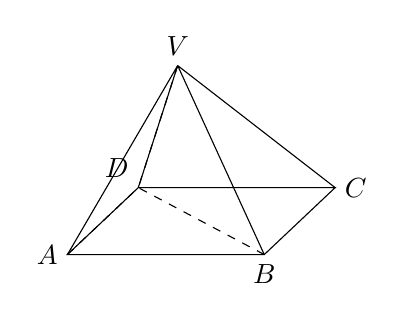
\begin{tikzpicture}[scale=1.0]
  \coordinate (V) at (0.1,2.4);
  \coordinate (A) at (-1.3,0);
  \coordinate (B) at (1.2,0);
  \coordinate (C) at (2.1,0.85);
  \coordinate (D) at (-0.4,0.85);
  \draw (V) -- (A) (V) -- (B) (V) -- (C) (V) -- (D);
  \draw (A) -- (B) -- (C) -- (D) -- cycle;
  \draw[dashed] (V) -- (D);
  \draw[dashed] (A) -- (D);
  \draw[dashed] (B) -- (D);
  \node[above] at (V) {$V$};
  \node[left] at (A) {$A$};
  \node[below] at (B) {$B$};
  \node[right] at (C) {$C$};
  \node[above left] at (D) {$D$};
\end{tikzpicture}
\end{center}
\nopagebreak[4]
\Needspace{4\baselineskip}
\textbf{解析}

\gksubpart{(1)}

平面 $VAD \perp$ 平面 $ABCD$ 且交线为 $AD$，底面内 $AB \perp AD$，故 $AB \perp$ 平面 $VAD$。

\gksubpart{(2)}

\Needspace{5\baselineskip}
设正方形边长 $2a$，取 $AD$ 中点 $O$ 为原点，$AD$ 为 $x$ 轴、$AB$ 方向为 $y$ 轴、面 $VAD$ 内垂直 $AD$ 方向为 $z$ 轴，则 $A(-a, 0, 0)$，$D(a, 0, 0)$，$B(-a, 2a, 0)$，$V(0, 0, \sqrt{3}a)$。平面 $VAD$ 的法向量为 $(0, 1, 0)$；平面 $VDB$ 由 $\overrightarrow{DV} = (-a, 0, \sqrt{3}a)$、$\overrightarrow{DB} = (-2a, 2a, 0)$ 张成，法向量取 $\vec{n} = (\sqrt{3}, \sqrt{3}, 1)$。于是
\nopagebreak[4]
\[
\cos\theta = \frac{\sqrt{3}}{\sqrt{3 + 3 + 1}} = \frac{\sqrt{21}}{7},
\]
二面角大小为 $\arccos\dfrac{\sqrt{21}}{7}$。

\gkanswer{答案（1）：由平面 $VAD \perp$ 底面及 $AB \perp AD$ 得 $AB \perp$ 平面 $VAD$。}

\gkanswer{答案（2）：$\arccos\dfrac{\sqrt{21}}{7}$。}

\end{answer}
\begin{answer}
\gksolhead{20}{}

\textbf{题目}：

在等差数列 $\{a_n\}$ 中，公差 $d \neq 0$，$a_2$ 是 $a_1$ 与 $a_4$ 的等比中项．已知数列 $a_1, a_3, a_{k_1}, a_{k_2}, \cdots, a_{k_n}, \cdots$ 成等比数列，求数列 $\{k_n\}$ 的通项 $k_n$．

\Needspace{4\baselineskip}
\textbf{解析}

由 $a_2$ 是 $a_1$ 与 $a_4$ 的等比中项得 $(a_1 + d)^2 = a_1(a_1 + 3d)$，即 $d^2 = a_1 d$，因 $d \neq 0$ 得 $a_1 = d$。于是 $a_n = nd$，$a_1 = d$，$a_3 = 3d$，公比 $q = 3$。故 $a_{k_n} = d\cdot 3^{n+1}$，即 $k_n d = 3^{n+1} d$，得 $k_n = 3^{n+1}$。

\gkanswer{答案：$k_n = 3^{n+1}$。}

\end{answer}
\begin{answer}
\gksolhead{21}{}

\textbf{题目}：

用长为 $90\ \mathrm{cm}$、宽为 $48\ \mathrm{cm}$ 的长方形铁皮做一个无盖的容器，先在四角分别截去一个小正方形，然后把四边翻转 $90^\circ$ 角，再焊接而成（如图），问该容器的高为多少时，容器的容积最大？最大容积是多少？
\nopagebreak[4]
\begin{center}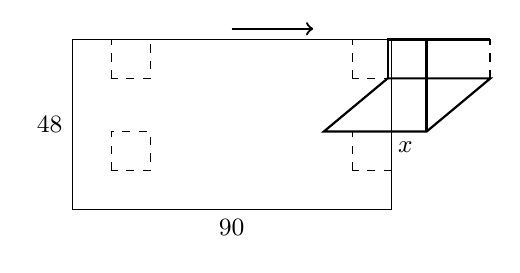
\begin{tikzpicture}[scale=0.9]
  \draw (0,0) rectangle (4.5,2.4);
  \foreach \x/\y in {0.55/0.55, 3.95/0.55, 0.55/1.85, 3.95/1.85}
    \draw[dashed] (\x,\y) rectangle ++(0.55,0.55);
  \draw[->, thick] (2.25,2.55) -- (3.4,2.55);
  \draw[thick] (3.55,1.1) -- (5.0,1.1) -- (5.9,1.85) -- (4.45,1.85) -- cycle;
  \draw[thick] (5.0,1.1) -- (5.0,2.4);
  \draw[thick,dashed] (5.9,1.85) -- (5.9,2.4);
  \draw[thick] (4.45,1.85) -- (4.45,2.4) -- (5.9,2.4);
  \node[below] at (2.25,0) {\small $90$};
  \node[left] at (0,1.2) {\small $48$};
  \node[below] at (4.7,1.1) {\small $x$};
\end{tikzpicture}
\end{center}
\nopagebreak[4]
\Needspace{4\baselineskip}
\textbf{解析}

\Needspace{5\baselineskip}
设截去的小正方形边长为 $x$（$0 < x < 24$），则容器高为 $x$，底面边长为 $90 - 2x$ 与 $48 - 2x$，容积
\nopagebreak[4]
\[
V(x) = x(90-2x)(48-2x) = 4x^3 - 276x^2 + 4320x.
\]
$V'(x) = 12x^2 - 552x + 4320 = 12\left(x^2 - 46x + 360\right)$，令 $V'(x) = 0$ 得 $x = 10$ 或 $x = 36$，由 $0 < x < 24$ 取 $x = 10$。此时 $V = 10\times 70\times 28 = 19600$。

\gkanswer{答案：高为 $10\ \mathrm{cm}$ 时容积最大，最大容积 $19600\ \mathrm{cm}^3$。}

\end{answer}
\begin{answer}
\gksolhead{22}{}

\textbf{题目}：

设 $A(x_1, y_1)$，$B(x_2, y_2)$ 两点在抛物线 $y = 2x^2$ 上，$l$ 是 $AB$ 的垂直平分线．

(1) 当且仅当 $x_1 + x_2$ 取何值时，直线 $l$ 经过抛物线的焦点 $F$？证明你的结论；

(2) 当 $x_1 = 1$，$x_2 = -3$ 时，求直线 $l$ 的方程．

\Needspace{4\baselineskip}
\textbf{解析}

\gksubpart{(1)}

\Needspace{5\baselineskip}
焦点 $F\left(0, \dfrac{1}{8}\right)$。设 $s = x_1 + x_2$，则 $AB$ 的斜率为 $\dfrac{2(x_2^2 - x_1^2)}{x_2 - x_1} = 2s$，中点为 $M\left(\dfrac{s}{2}, x_1^2 + x_2^2\right)$。$l$ 过 $F$ 等价于 $\overrightarrow{FM} \perp \overrightarrow{AB}$：
\nopagebreak[4]
\[
\left(-\frac{s}{2}\right)\left(x_2 - x_1\right) + \left(\frac{1}{8} - x_1^2 - x_2^2\right)\cdot 2s\left(x_2 - x_1\right) = 0,
\]
即 $s\left[-\dfrac{1}{4} - 2\left(x_1^2 + x_2^2\right)\right] = 0$。因括号内恒为负，故当且仅当 $s = 0$（此时 $l$ 为 $x = 0$，恰过 $F$）。

\gksubpart{(2)}

$x_1 = 1$，$x_2 = -3$ 时 $A(1, 2)$，$B(-3, 18)$，中点 $(-1, 10)$，$AB$ 斜率为 $-4$，故 $l$ 的斜率为 $\dfrac{1}{4}$，方程为 $y - 10 = \dfrac{1}{4}(x + 1)$，即 $x - 4y + 41 = 0$。

\gkanswer{答案（1）：当且仅当 $x_1 + x_2 = 0$ 时直线 $l$ 经过焦点 $F$。}

\gkanswer{答案（2）：$x - 4y + 41 = 0$。}

\end{answer}